\documentclass[tikz,border=10pt]{standalone}
\begin{document}
\usetikzlibrary{arrows.meta, shadows, fadings,shapes.arrows}
\tikzset{My Arrow Style/.style={single arrow, fill=red!50, anchor=base, align=center}}

\begin{tikzpicture}
    \node[anchor=south west,inner sep=0] at (0,0) (craters) {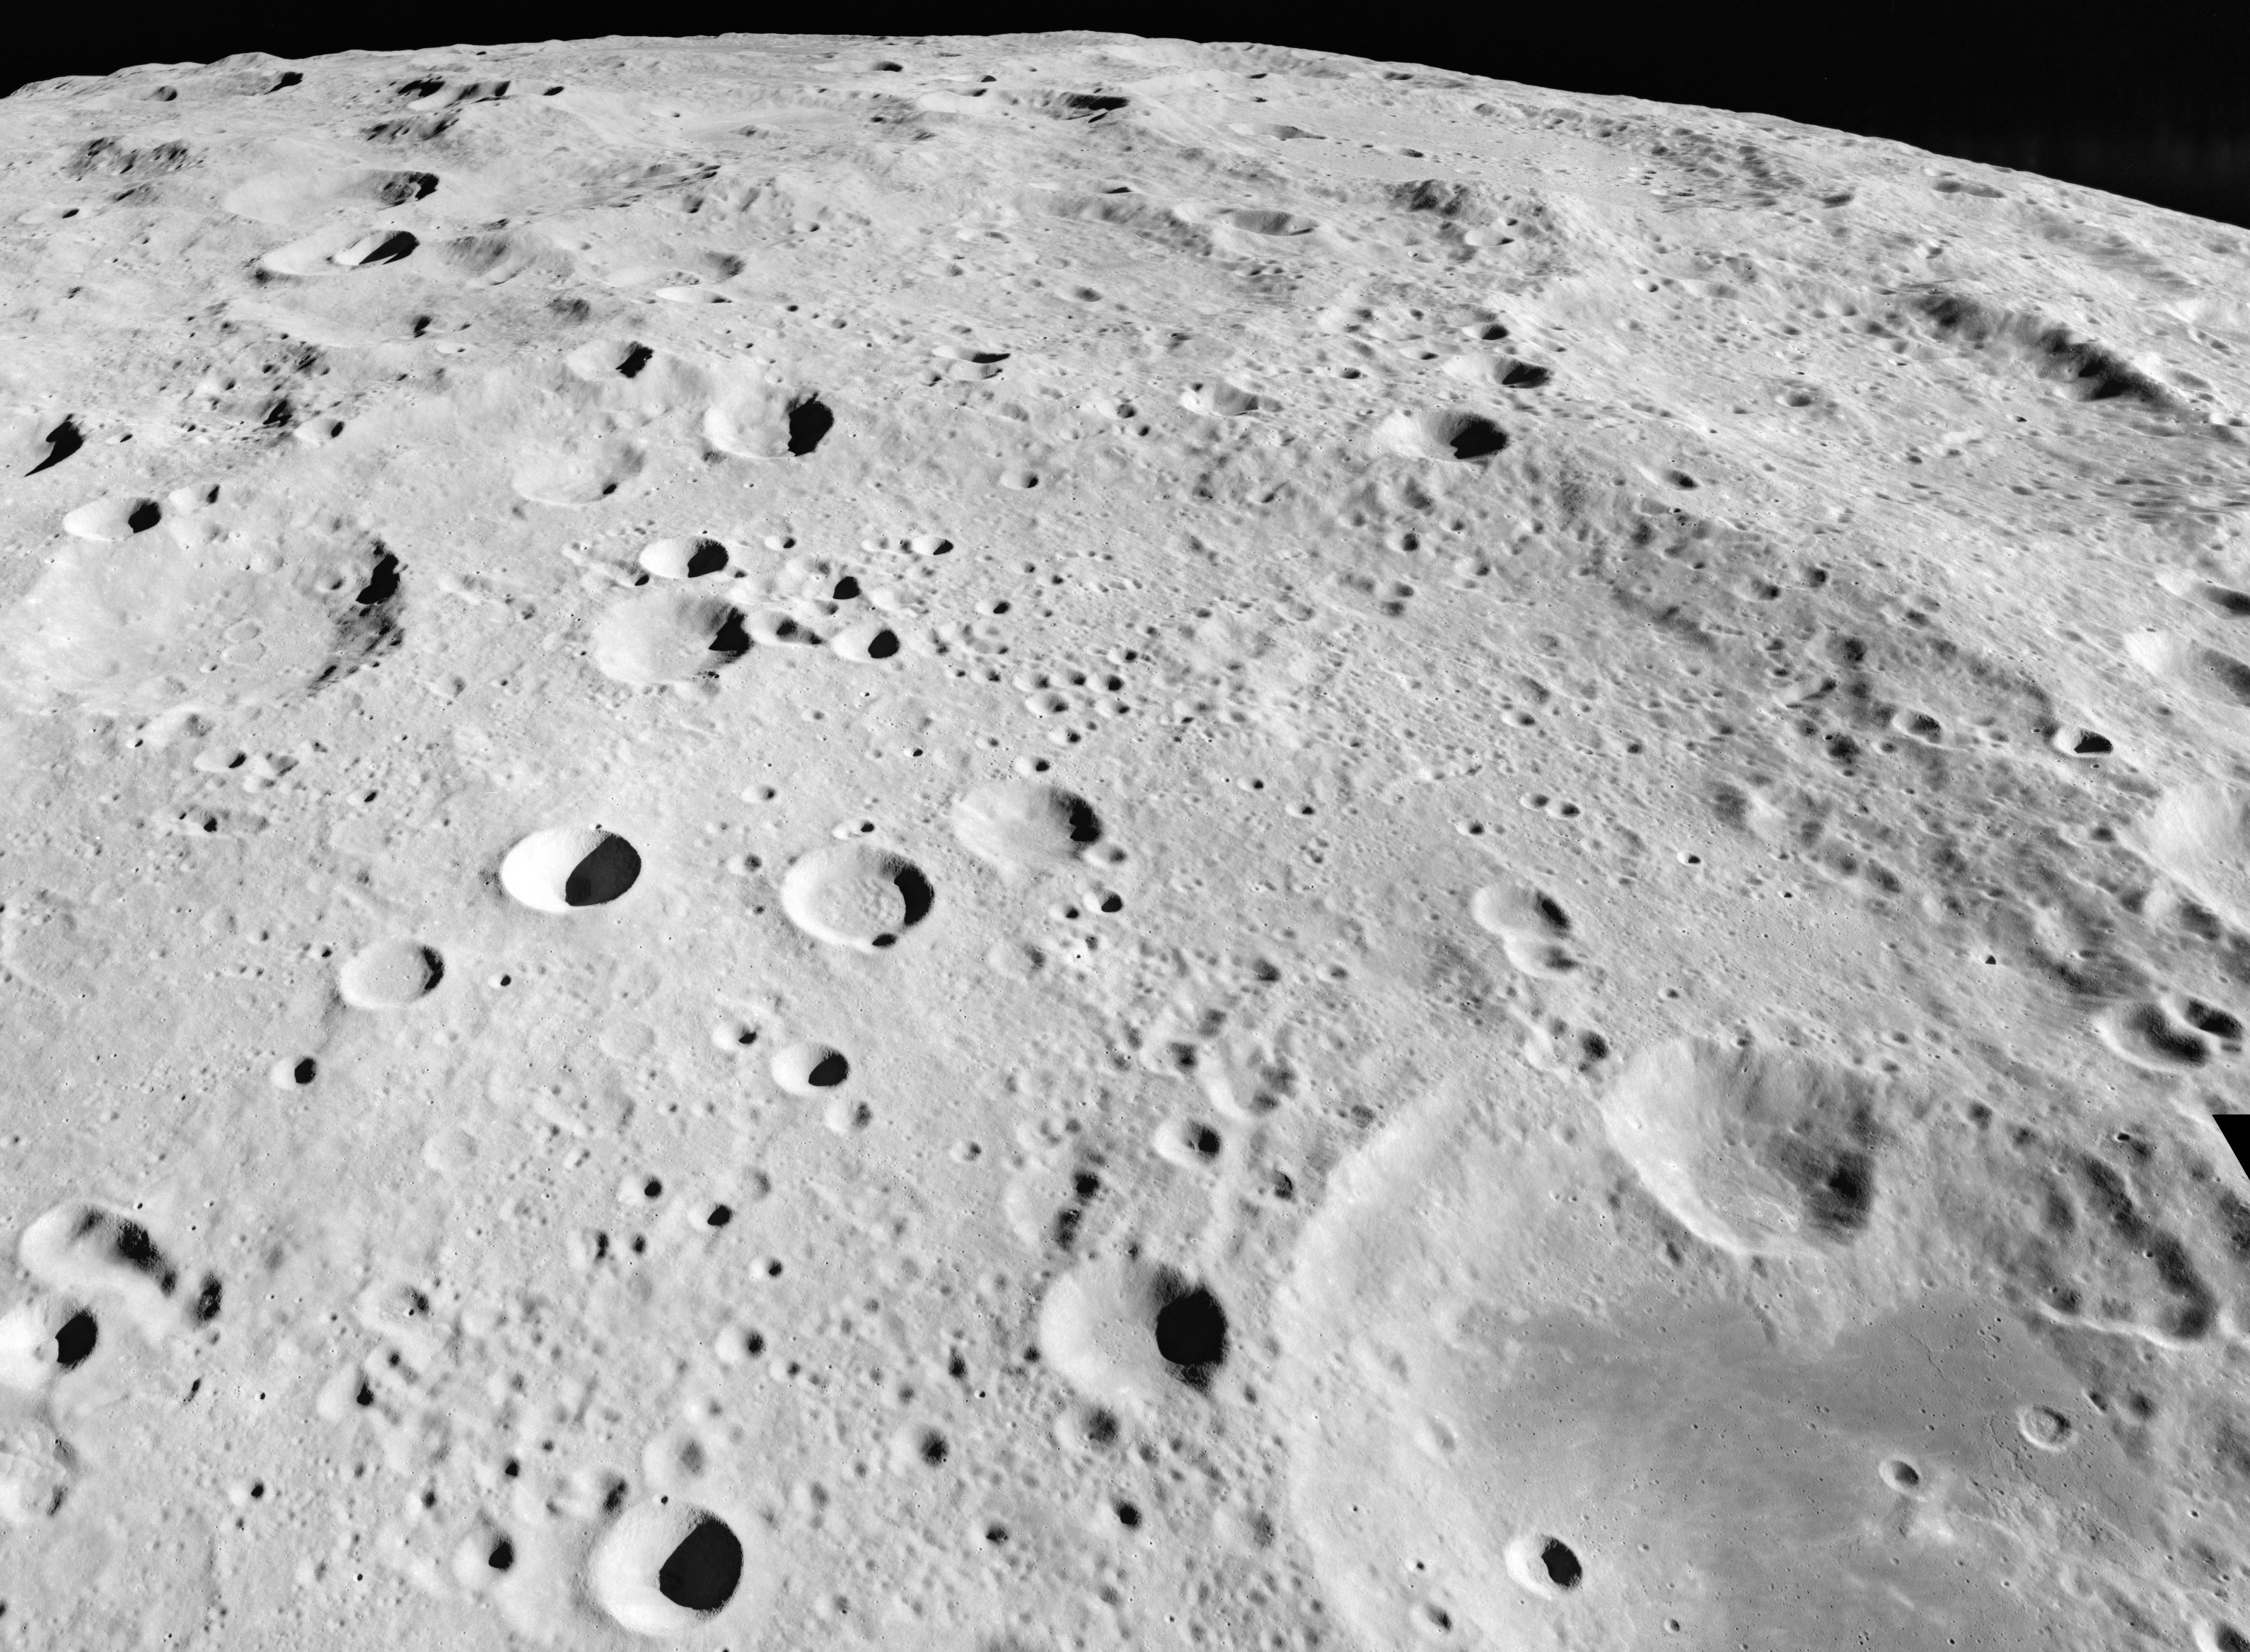
\includegraphics[width=\textwidth]{Gagarin_crater_AS17-M-1565_corner.jpg}};
    \node[red,anchor=south west,align=left, shape=rectangle, fill=white] at (0,0) (extraction) { feature extraction };
    \draw[red,thick] (3.1,4.23) ellipse (3.8mm and 2.2mm);
    \draw[red,thick] (7.9,6.55) ellipse (2mm and 1mm);
    \draw[red,thick] (3.6,0.46) ellipse (3.9mm and 3.3mm);
    \draw[red,thick] (3.1,4.23) -- (13,4.5);
    \draw[red,thick] (7.9,6.55) -- (13,4.5);
    \draw[red,thick] (3.6,0.46) -- (13,4.5);
    \node[align=center] at (13.9,4.5) (features) { feature \\ descriptors };
    \node[My Arrow Style] at (16.0, 4.2) (matching) {feature \\ matching};
    \node[align=left] at (19.0, 4.6) (position) { \Large\itshape positions in \\ \Large\itshape lunar-fixed \\ \Large\itshape frame};
\end{tikzpicture}
\end{document}